\documentclass[letterpaper, 10pt, conference]{ieeeconf}
\usepackage{graphicx, amsmath, amsfonts, mathtools} 
\usepackage{units}
\usepackage{color}
\date{}
\graphicspath{ {./figs/} }

% \makeatother

\title{Gas Injection System modelling and control for ITER}
\author{\authorblockN{Dante Piotto\authorrefmark{1},
                        Anna Trang Vu\authorrefmark{2},
                        Luca Zabeo\authorrefmark{2}, 
                        Laurent Lef\`evre\authorrefmark{3}, 
                        Alessandro Macchelli\authorrefmark{1}, \\
                        Thomas Keenan\authorrefmark{2}, 
                        Remy Nouailletas\authorrefmark{4},
                        Timo Ravensbergen\authorrefmark{2},                          
                        Peter De Vries\authorrefmark{2},                        
                        David Weldon\authorrefmark{4}}\\
	\authorrefmark{1} Univ.  of Bologna, DEI, viale del Risorgimento 2, Bologna, Italy\\ %\{firstname.lastname\}@}
	\authorrefmark{2} ITER Organization, Route de Vinon-sur-Verdon, 13067 St. Paul Lez Durance Cedex, France \\%\{firstname.lastname\}@iter.org}
	\authorrefmark{3} Univ. Grenoble Alpes, Grenoble INP, LCIS, 26000 Valence, France \\ %\{firstname.lastname\}@lcis.grenoble-inp.fr}
    \authorrefmark{4} CEA, IRFM, 13108 St-Paul-Lez-Durance, France %\{firstname.lastname\}@cea.fr}
    }
\begin{document}


\maketitle
\thispagestyle{empty}
\pagestyle{empty}

\begin{abstract}

This article presents the modelling and control of the ITER Gas Injection System. The non-linear models for both the valve and the pipe are formulated using the port-Hamiltonian approach. The primary focus of this study is the valve model, which incorporates both the mechanical and electrical domains, as well as the nonlinear coupling between them. An observer is designed for the valve to reconstruct the system states from the gas flow measurement at the valve output. A passivity-based controller is then developed to regulate gas flow into tokamak vacuum vessel. The valve model is implemented in the ITER simulation platform PCSSP and validated with experimental data. The control algorithm is implemented and tested in simulation.

\end{abstract}
\section{Introduction}
The ITER Gas Injection System (GIS)\cite{GIS_2012} is the system responsible for supplying gas to the vacuum vessel, mainly for fuelling and plasma radiation enhancement purposes. It will play a key role in the plasma density control performed by the Plasma Control System (PCS) \cite{deVries2024}. This work focuses on the modelling and control of the ITER GIS, with particular attention to the valves that supply gas to the vacuum vessel. The main challenge in control of the GIS is given by the significant delay introduced into the system by the length of the pipes from 17 to 40 m connecting the fuelling valves to the vacuum vessel.

% add motivation from Michael Walsh's comment
From a practical perspective, this diffusion system can be viewed as a basic proportional model with an associated delay. However, the delay is not constant and varies based on several factors, including the type of gas valve, the specific gas species, temperature, and more. Additionally, the delay is further influenced by the length of the pipe. As a result, the delay observed from experimental data may not fully capture the system’s behavior, particularly under varying control commands, such as those used for density control. Therefore, this study proposes the development of precise models and an advanced control algorithm to ensure the optimal performance of the GIS.
The port-Hamiltonian approach \cite{maschke1993port,schaft2020}, with its modular feature and stability analysis advantages, is an appropriate method for modelling of multiphysic systems, such as the GIS. Different from the levitated ball system in \cite{schaft2020}, Sec.2.6, non-linear coupling is considered between the mechanical and electrical domains in this application.

The control strategy Interconnection and Damping Assignment - Passivity Based Control (IDA-PBC) proposed in this paper was initially presented in \cite{IDAPBC}. Control of a similarly class of the considered systems has been discussed in \cite{PHintro, weakcouple}. 
% The solutions in the aforementioned rely on the linear structure of the considered systems, which is not present in the case discussed in this paper. ==> A.Vu: What does it mean?
In \cite{integralIDA} it is shown that integral control can be combined with the IDA-PBC technique to improve robustness of the control. 
This model-based control technique requires complete knowledge of the system states. To achieve this, an observer is designed for the valve to reconstruct these states using the gas flow measurements taken at the valve output.

The proposed valve model is implemented in the ITER simulation platform PCSSP \cite{Ravensbergen2023} and validated with experimental data from the testbench at the South Western Institute of Physics (SWIP). The control algorithm is implemented and tested in simulation.
 
The rest of the paper is organized as follows: section \ref{sec:overview} gives an overview of the ITER GIS and the proposed control scheme, section \ref{sec:vlvmdl} describes the modelling of the valves in the GIS and displays the obtained results, section \ref{sec:pipemdl} describes the adopted model for the pipes connecting the valves to the vacuum vessel, section \ref{sec:ctrl} describes the proposed control scheme and displays its performance in simulation, and lastly section \ref{sec:conclusion} concludes the paper.

\section{ITER GIS overview and control scheme}\label{sec:overview}
The GIS is composed of 10 Gas Valve Boxes (GVB),  6 at the divertor (bottom) level and 4 at the upper port level, (see Fig. \ref{fig:GIS}) \cite{GIS_2012}. Each GVB consisting of 6 Mass Flow Controlled (MFC) valves for different species, and the pipe system connecting the GVBs to the vacuum vessel (VV), Fig. \ref{fig:GIS_scheme}.
\begin{figure}[!ht]
     \centering
     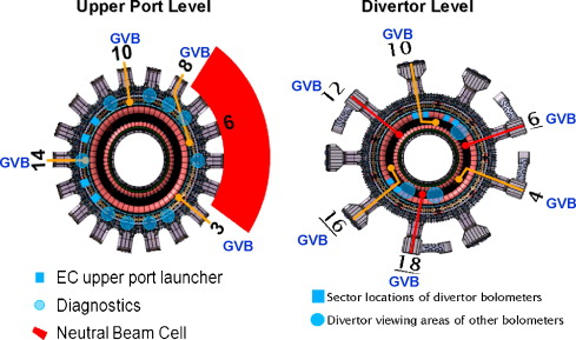
\includegraphics[width=0.45\textwidth]{GIS_ip}
     \caption{Location of 10 GVBs and injection points in the ITER Vacuum Vessel \cite{GIS_2012}}
     \label{fig:GIS}
\end{figure}
\begin{figure}[!ht]
     \centering
     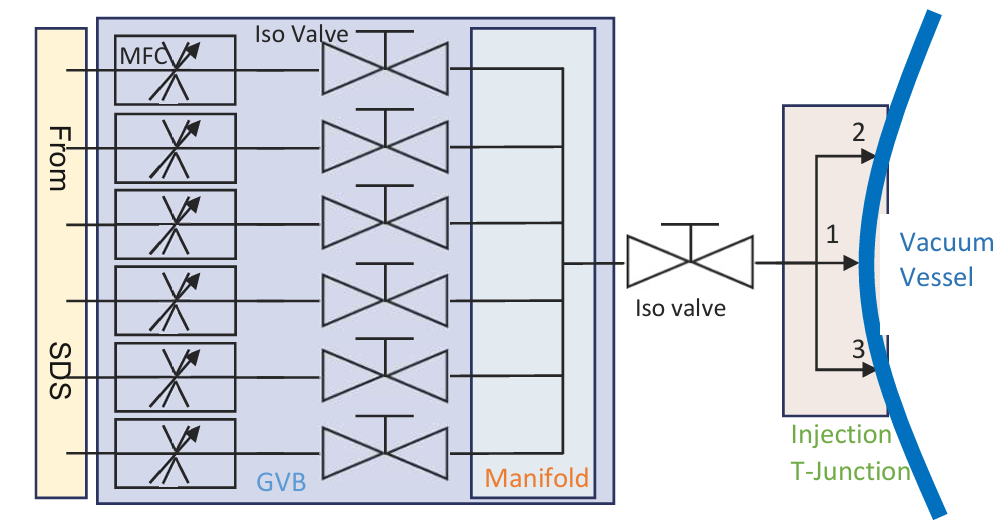
\includegraphics[width=0.35\textwidth]{GIS_scheme.png}
     \caption{GIS scheme includes 1 GVB, pipeline (17-40 m) and different injection points into the vacuum vessel}
     \label{fig:GIS_scheme}
\end{figure}
\begin{figure}[!ht]
    \centering
    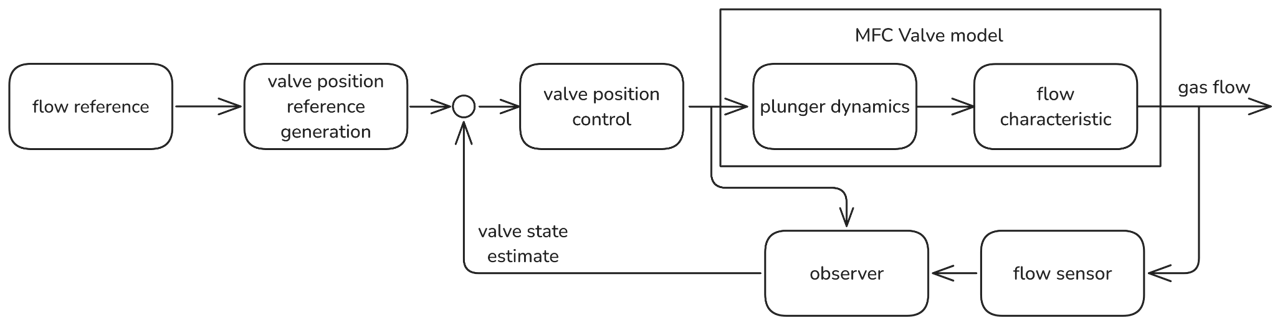
\includegraphics[width=0.49\textwidth]{ctrl_scheme}
    \caption{Proposed control scheme for the MFC valves}
    \label{fig:ctrlscheme}
\end{figure}

In order to control the flow output of the MFC by regulating the voltage input of the plunger, we propose the following control scheme Fig. \ref{fig:ctrlscheme}. In the next section, we will develop a control-oriented model per block in the scheme, and validate the model against SWIP experimental data.

\section{MFC Valve model}\label{sec:vlvmdl}
The MFC valves in the ITER GIS are solenoid actuated, normally closed valves, Fig. \ref{fig:valvesec}. 
The dynamic model of the valves was divided into two main components: an electromechanical model for the the solenoid, and a flow characteristic that relates mechanical variables of the system to gas flow out of the valve.
\subsection{Plunger dynamics model} \label{sec:plung}
The linear solenoid actuator that operates the valve is modelled through the interaction of two subsystems: a mass-spring-damper, representing the mechanical portion of the actuator, and an RL circuit, for the electric part of the actuator. 
The interaction between these two subsystems is of electromagnetic nature. As the ferromagnetic plunger within the solenoid moves, the inductance of the RL cuircuit changes, and a magnetic force is exerted on the mass-spring-damper system based on the current flowing through the inductor. Following the port-Hamiltonian approach \cite{PHintro}, we may develop models for the two subsystems and then connect them.
\begin{figure}[!ht]
    \centering
     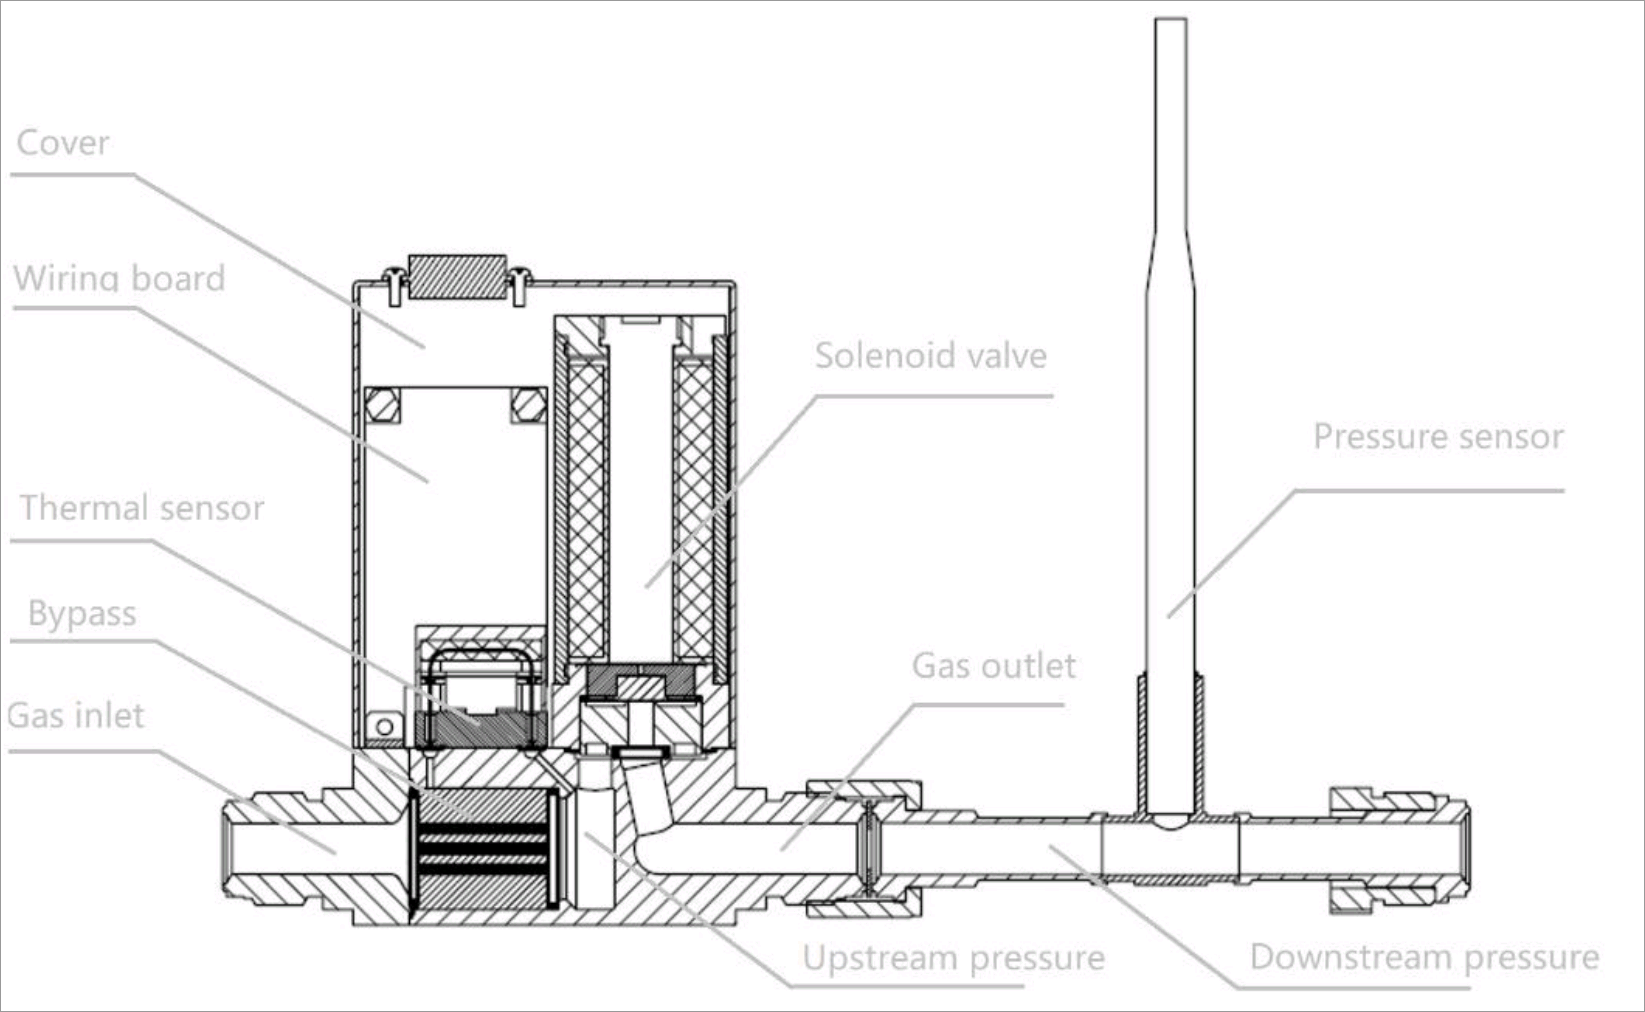
\includegraphics[width=0.4\textwidth]{valvesection}
     \caption{Side section of an MFC valve}
     \label{fig:valvesec}
\end{figure}
\subsubsection{Mechanical subsystem}
The Hamiltonian for the mechanical subsystem is the sum of elastic and kinetic energy:
\begin{align}
H_m(q,p) = \frac{1}{2}kq^2 + \frac{1}{2m} p^2  
\end{align}
where $q$ is the position of the plunger and $p$ is its momentum, $k$ is the spring constant and $m$ is the mass of the plunger.
The interconnection and damping matrices are:
\begin{align}
J_m = \begin{bmatrix}
    0 & 1 \\ -1 & 0
\end{bmatrix} \quad R_m = \begin{bmatrix}
    0 & 0 \\ 0 & b
\end{bmatrix}
\end{align}
where $b$ is the damping coefficient.
The dynamic equations for the mechanical subsystem are then
\begin{align}
\dot{x}_m = [J_m-R_m]\frac{\partial H_m}{\partial x_m}
\end{align}\label{original_PCH}
where $x_m = \begin{bmatrix}
    q & p 
\end{bmatrix}^\top $ is the state of the mechanical subsystem

\subsubsection{electrical subsystem}
The Hamiltonian for the electrical subsystem is composed only of the energy stored in the solenoid coil, using as state the flux linkage in the inductor:
\begin{align}
H_e(\varphi) = \frac{\varphi}{2 L}
\end{align}
Interconnection and damping are trivial:
\begin{align}
J_e = 0 \quad R_e = R_c
\end{align}
with $R_c$ the resistance of the RL circuit.
The electrical subsystem presents an input voltage, thus the dynamic equation presents as:
\begin{align}
    \dot{x}_e = [J_e-R_e]\frac{dH_e}{dx_e} + gu
\end{align}
with $g=1$ and $u=v_{in}$ the input voltage
\subsubsection{Inductance function}
The relation between position of the plunger in the solenoid and inductance is rather complex in its nature, and analytic expressions can be quite involved \cite{analytic_solen}. For this reason, an approximation of the inductance function based on the experimental work in \cite{approx_solen} is used:
\begin{equation}
    L(q) = A\left(1 + \frac{q}{c+q}\right)
\end{equation}

\subsubsection{Coupling the subsystems}
Following PH system theory the mechanical and electromechanical subsystems can be interconnected by considering a state space composed of the cartesian product of the state spaces of the subsystems, a Hamiltonian constructed as the sum of the subsystem Hamiltonians and interconnection and damping matrices composed with those of the subsystems. Dependance of the inductance on the plunger position gives the coupling between the mechanical and electrical physical domains.
\begin{align}
    &H(q,p,\varphi) = H_m + H_e = \frac{1}{2}kq^2 + \frac{1}{2m} p^2 + \frac{\varphi}{2 L(q)}\\
    &J = \begin{bmatrix}
        J_m & 0 \\ 0 & J_e
    \end{bmatrix}  = \begin{bmatrix}
        0 & 1 & 0 \\ 
        -1 & 0 & 0 \\
        0 & 0 & 0
    \end{bmatrix}\\
    &R = \begin{bmatrix}
        R_m & 0 \\ 0 & R_e
    \end{bmatrix} = \begin{bmatrix}
        0 & 0 & 0 \\
        0 & b & 0\\
        0 & 0 & 0
    \end{bmatrix}
\end{align}
The dynamic equations of the system can be expressed as

\begin{equation}
    \dot{x} = [J-R]\frac{\partial H}{\partial x} + gu \label{eq:plunger_original_PCH}
\end{equation}
with $x = \begin{bmatrix}
    x_m & x_e
\end{bmatrix}^\top$, $g=\begin{bmatrix}
    0 & 0 & 1
\end{bmatrix}^\top$ and $u=v_{in}$

\subsection{Flow characteristic approximation model}\label{sec:flow_charac}
The valve is approximated as varying conductance between two pipes. The particle flow, expressed in $[\unit{Pa\,m^{3}\,s^{-1}}]$ is given by Bernoulli's equation:
\begin{align}
    Q = \frac{RT}{M} \frac{C_d}{\sqrt{1-\beta^4}}\varepsilon\frac{\pi}{4}d^2\sqrt{2(P_{up}-P_{down})\rho}
\end{align}
many of these parameters are unknown, and are therefore aggregated into a single one, yielding the following expression:
\begin{align}
    Q = \xi_{gas}C_d\sqrt{\left(P_{up}^2-P_{down}^2\right)}
\end{align}
The parameter $\xi_{gas}$ is tuned so that with $C_d=1$ the flow out of the valve matches what observed from the experimental tests where the valve is fully opened. 
The discharge coefficient $C_d\in[0,1]$ is a function of the plunger position $q$. This function is identified by attempting to bridge the gap between experimental data and the mathematical model developed so far.
\subsection{Flow sensor model}
The MFC valve is equipped with a sensor to measure the flow rate, schematized in Fig. \ref{fig:sensor}. Part of the gas flowing through the valve flows through the sensor. The gas stream through the sensor is warmed up by two heaters ($\text{R}_{\text{HT1}}$ and $\text{R}_{\text{HT2}}$). When the valve is open, the gas transports heat from the first resistor to the second, causing a temperature difference between the two resistors, which is linearly dependent to mass flow rate \cite{sensor}:
\begin{align}
    \dot{m} = \alpha \Delta T
\end{align}
\begin{figure}[!htb]
    \centering
    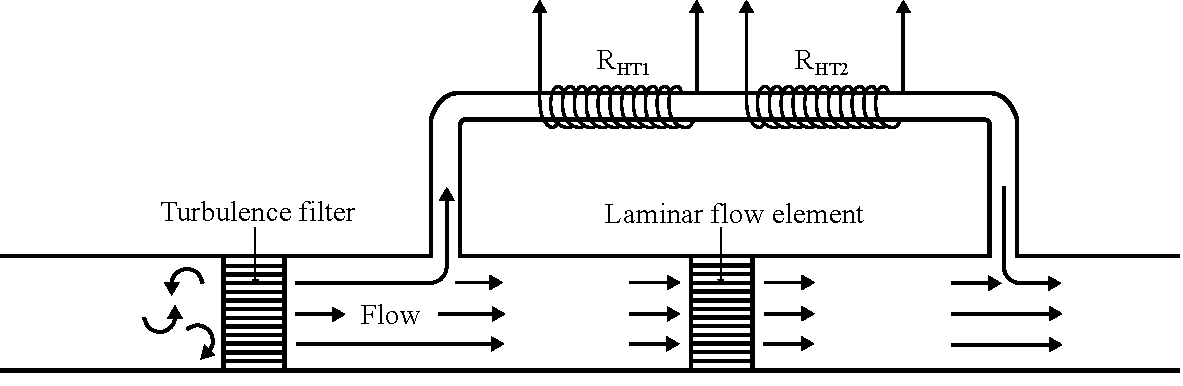
\includegraphics[width = 0.8\columnwidth]{flow_sensor}
    \caption{Schematic of the MFC valve flow meter}
    \label{fig:sensor}
\end{figure}
Due to the physical phenomenon on which the sensor is based (heat transfer in a moving gas), the sensor presents a delayed response, which can be observed in experimental data as a time delay between the effect of opening the valve on sensed flow downstream of the valve. % as shown in Figure \ref{fig:sensslow}.
%\begin{figure}[!htb]
%    \centering
%    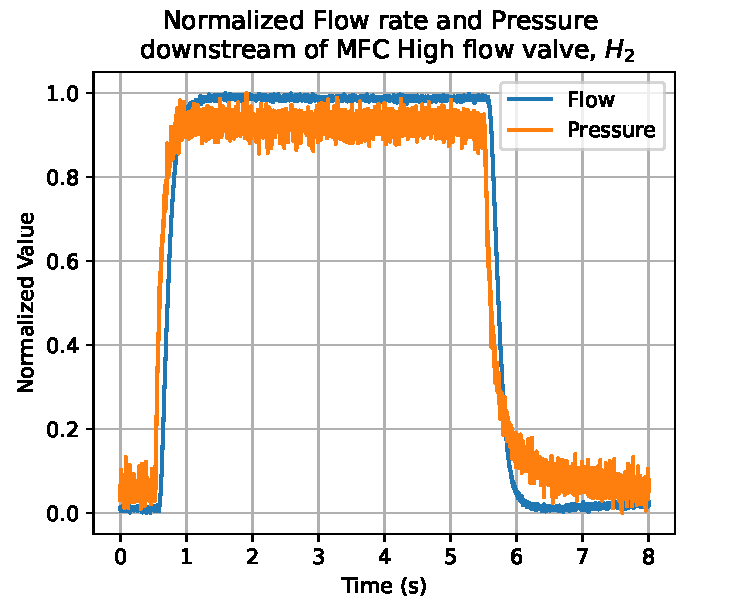
\includegraphics[width = 0.45\textwidth]{D7_flow_press.pdf}
%    \caption{Comparison of flow sensor data with pressure downstream of MFC valve}
% * <vu.nmtrang@gmail.com> 10:38:50 11 Feb 2025 UTC+0100:
% not clear what to compare here, should be both for flow, from different sensors.
%    \label{fig:sensslow}
%\end{figure}

Since the a physical model for the sensor is too complicated for the scope of this paper, it was instead approximated as a simple low-pass filter applied to the mass flow rate through the valve, with its parameters determined experimentally. In particular, a Bessel filter was used due to its property of providing constant group delay in the passband \cite{filtering}.
The cutoff frequency for the low-pass filter can be expected to depend on properties of the gas being considered --- molar mass, flow rate, temperature, etc. In this case temperature is assumed to always be the same, while gas species and flow rates clearly vary. In particular, heavier gases flowing slower will make for slower sensing. A different cutoff frequency was tuned for each gas-valve pairing to account for this.

\subsection{Comparison of the simulation model with experimental data}
% Alessandro: I would put a sentence that explains how the parameters are determined from data
% * <vu.nmtrang@gmail.com> 17:12:56 13 Mar 2025 UTC+0100:
% if space allows
The MFC valve model, including the plunger dynamics and the flow characteristic, with and without the flow sensor model has been validated against experimental data gathered on a testbench by SWIP, for different gas species, Fig. \ref{fig:mdl_H2} for $H_2$ and Fig. \ref{fig:mdl_Ar} for $Ar$, with different feedforward references of the input voltage. The results of simulation flow, red curves in the figures, represent the ideal flow at the MFC output, while the results of flow after sensor, green curves, take into account the delay due to the sensor measurement. The simulation results with simulated sensor match very well the experimental results. 
% * <vu.nmtrang@gmail.com> 11:16:26 11 Mar 2025 UTC+0100:
% I add some comments here to explain the figures

\begin{figure}[!ht]
    \centering
    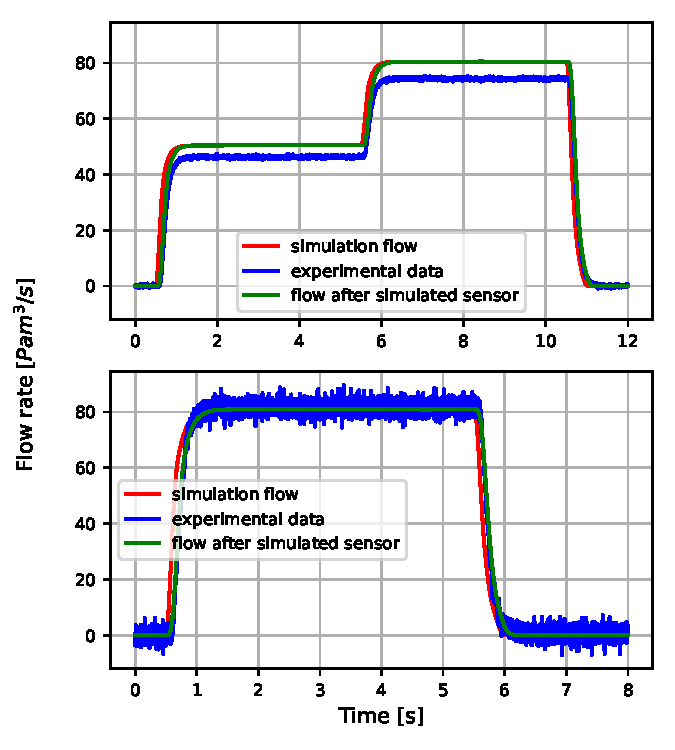
\includegraphics[width=0.4\textwidth]{H2_model.pdf}
    \caption{Comparison of simulated high flow valve with experimental data for $H_2$ }
    \label{fig:mdl_H2}
\end{figure}

\begin{figure}[!ht]
    \centering
    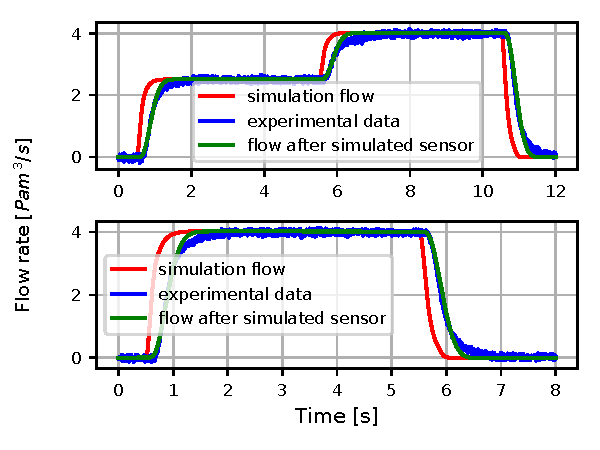
\includegraphics[width=0.4\textwidth]{Ar_model.pdf}
    \caption{Comparison of simulated high flow valve with experimental data for $Ar$}
    \label{fig:mdl_Ar}
\end{figure}


\section{Pipe model}\label{sec:pipemdl}
% Alessandro: the ports of the pipe model are not shown, thus it is complicated to understand how to include it into the complete model (see also the final part of the paper). If you work with port-Hamiltonian systems, the “interface” should be specified. 
% * <vu.nmtrang@gmail.com> 17:12:34 13 Mar 2025 UTC+0100:
% good point, add the boundary condition if possible
The pipe connecting the valve to the vacuum vessel is modelled by a 1D diffusion PDE:
\begin{equation}
    \begin{aligned}
    Q_k(x,t) &= - C_k(x,t)\partial_x P_k(x,t) \\
    \partial_t P_k(x,t) &= -\frac{1}{A} \partial_x Q_k(x,t)
    \end{aligned}
\end{equation}
where the pipe conductance $C_k = C_{k-molecular}+C_{viscous}$ is composed of a molecular and viscous component. The molecular component is computed as
\begin{equation}
    C_{k-molecular} = \frac{\pi}{12}\bar{v}_kd^3 \qquad \bar{v}_k = \sqrt{\frac{3RT}{M_k}}
\end{equation}
with $d$ the pipe diameter, $\bar{v}_k$ the molecular velocity, $R$, $T$, and $M_k$ respectively the perfect gas constant, the gas temperature and molar mass of gas species $k$. Viscous conductance is computed as:
\begin{equation}
    C_{viscous} (x,t) = \frac{\pi R_0^4}{8\eta(x,t)} \sum_k P_k(x,t)
\end{equation}
where $R_0$ is the pipe radius and $\eta(x,t)$ is the viscous friction:
\begin{equation}
    \eta^{-1}(x,t) = \eta_k^{-1} \frac{M_k P_k(x,t)}{\displaystyle\sum_k M_k P_k(x,t)} 
\end{equation}
where $\eta_k$ is the viscosity of each single gas, computed with Sutherland's formula:
\begin{equation}
    \eta_k = \eta_{k-0} \frac{T_{k-0} + C_k\prime}{T + C_k\prime}\frac{T^{3/2}}{T_k^{3/2}}
\end{equation}
where $\eta_{k-0}$, $T_{k-0}$ and $c_k\prime$ are respectively the reference viscosity, the reference temperature and Sutherland's constant for the gas species.

The pipe model presents four boundary variables: molecular flow rate  and pressure at the boundaries of the pipe. Of these, flow at the pipe inlet and pressure at the pipe outlet are set as input variables, while pressure at the inlet and flow at the outlet are set as output variables.

The model is implemented in simulation through a finite-difference method.

\section{Control Design}\label{sec:ctrl}
The control scheme for the valve is composed of two main components: an observer to reconstruct the state of the valve, and a controller that uses this information to steer the system to a desired setpoint or trajectory. Both the observer and the control law have been implemented in discrete-time in accordance with the requirements for the ITER Control System. It is to be noted that the controller was developed with the assumption that the state of the valve be known, thus creating the need for an observer to infer such information.
% * <vu.nmtrang@gmail.com> 10:39:31 11 Feb 2025 UTC+0100:
% explain that observer itself is not taken into account  in the control design algo. Only the observer result is used 

\subsection{Observer}
In order to build the observer, the system state is extended by adding the flow rate measured by the flow sensor as it has dynamic behaviour w.r.t the state of the plunger, and is renamed $\xi = [x \ Q_m]^\top$ with $Q_m$ the measured flow rate.
The chosen structure for the observer is that of a Luenberger observer with added integral action:
\begin{align}
    \hat{\xi}_{k+1} = f_d(\hat{\xi}_k, u_k) + K_P(\hat{y}-y) + K_I \displaystyle\sum_{t=0}^{k}(\hat{y}-y)
\end{align}
where $f_d$ is the discretized valve dynamics, obtained through the Runge-Kutta method for the plunger dynamics, and through the least-squares method using MATLAB's \verb|c2d()| function to discretize the Bessel filter transfer function for the sensor dynamics. 

%In Figure \ref{fig:flowhat} the behaviour of the observer with white noise on the flow measurement is displayed for a high flow valve, while in Figure \ref{fig:flowhat_F} the behaviour of the observer when a force step is applied to the plunger at $t=3s$ can be seen.
%As can be seen in the disturbed case (Fig. \ref{fig:flowhat_F}) plunger momentum and flux linkage estimates do not converge to the real values. This is not a problem as the controller only needs to ensure that the plunger position reaches its reference to achieve the desired flow rate.
The observer can perfectly estimate the system state with white noise on the flow measurement. With a disturbance of a force step applied to the plunger at $t=3s$ in Fig. \ref{fig:flowhat_F}, plunger momentum and flux linkage estimates do not converge to the real values. However, this offset does not impact the control effect, as the control law relies solely on the plunger position.

%\begin{figure}[!ht]
%    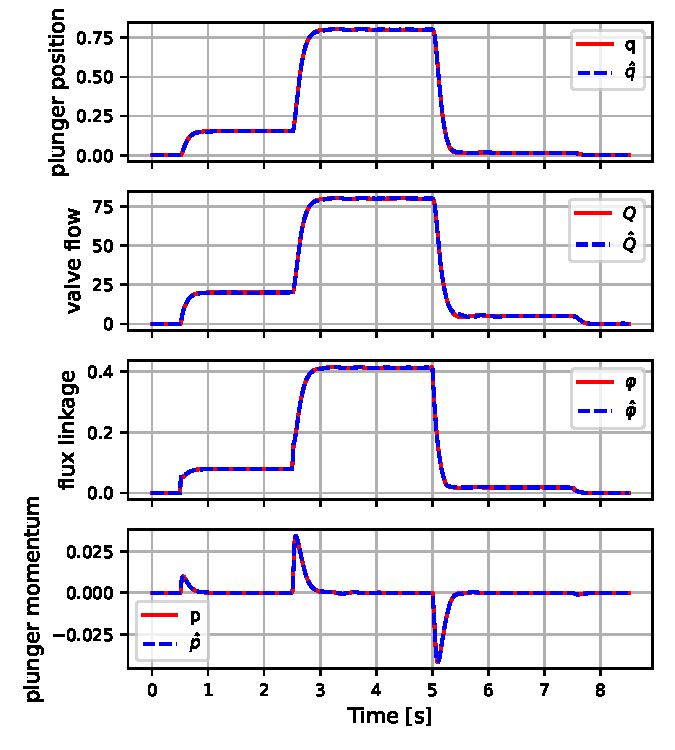
\includegraphics[width=0.48\textwidth]{combined_plots_obs.pdf}
%    \caption{Observer estimates of valve states}
%    \label{fig:flowhat}
%\end{figure}

\begin{figure}[!ht]
    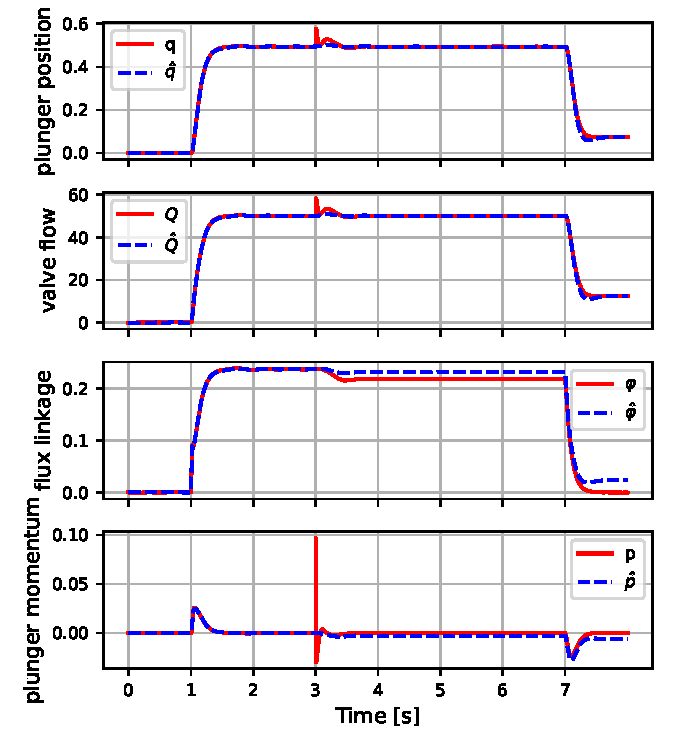
\includegraphics[width=0.48\textwidth]{combined_plots_obs_F.pdf}
    \caption{Observer estimates of valve states with disturbance step at $t=3s$}
    \label{fig:flowhat_F}
\end{figure}

\subsection{Reference Generation}
% * <vu.nmtrang@gmail.com> 16:02:51 10 Feb 2025 UTC+0100:
% may put this subsec before the controller design?
The designed controller is focused on regulating the plunger subsystem, tracking references for the plunger state as outlined in subsection \ref{sec:plung}. It is important to note that reference for the system is provided in terms of flow rate, while the reference for the plunger subsystem is the valve position. As a result, it is necessary to convert the flow reference into corresponding reference for the plunger state. This can be achieved by inverting the valve’s flow characteristic, \ref{sec:flow_charac} to determine the desired plunger position. The open-loop valve dynamics can then be solved to find the required steady-state flux linkage, and for static references, the desired momentum will be zero.

\subsection{Valve position control using IDA-PBC}
Control is developed for the plunger model, the electromechanical subsystem described in subsection \ref{sec:plung}.
By taking advantages of the PCH formulation of the plunger model, the chosen control scheme is IDA-PBC \cite{IDAPBC}, following the Algebraic approach to solving the matching equation. The main idea is to `transform' the original system \eqref{eq:plunger_original_PCH} to a target PCH system via the control input $u$. 
\begin{equation}
    \begin{aligned}
    \dot{x} &=& [J-R]\frac{\partial H}{\partial x} + gu &=& [J_{d}- R_{d}]\frac{\partial H_{d}}{\partial x}
\end{aligned}\label{eq:IDA_principle}
\end{equation}

A quadratic energy function which has the minimum at the equilibrium is selected as the target Hamiltonian:
\begin{align}
    H_d(q,p,\varphi) = \frac{\gamma_1}{2} (q-q^\star)^2 + \frac{p^2}{2m} + \frac{\gamma_2}{2}(\varphi-\varphi^\star)^2
    \label{eq:Hd}
\end{align}
A general form for the desired interconnection skew symmetric ($J_d$) and non negative damping ($R_d$) matrices is considered at first, along with a trivial option for the left annihilator of $g$:
\begin{equation}
    \begin{aligned}
    J_{d}(x) &= \begin{bmatrix}
        0 & J_{1,2} & J_{1,3}\\
        -J_{1,2} & 0 & J_{2,3}\\
        -J_{1,3} & -J_{2,3} & 0
    \end{bmatrix} \quad R_{d}(x) = \begin{bmatrix}
        r_{1} & 0 & 0\\
        0 & r_{2} & 0\\
        0 & 0 & r_{3}\\
    \end{bmatrix} \\
    g^\perp &= \begin{bmatrix}
        1 & 0 & 0\\ 
        0 & 1 & 0
    \end{bmatrix}
\end{aligned}\label{eq:JRd}
\end{equation}
% Alessandro: I would try to add a stability proof. Since the target is a journal and a rather theoretical conference, stating a result without a proof could be a risk.
The stability of the closed loop is trivial:
\begin{equation}
    \begin{aligned}
    \dot{H_{d}} = \frac{\partial^T H_{d}}{\partial x} \dot{x} &=& -\frac{\partial^T H_{d}}{\partial x} R_{d}\frac{\partial H}{\partial x}  \leq 0
\end{aligned}\label{eq:IDA_stab}
\end{equation}

The matching condition \eqref{eq:IDA_principle} between the original system and the target closed loop system characterised by (\ref{eq:Hd}-\ref{eq:JRd}) thus yields a set of two equations:
\begin{equation}
    \begin{aligned}
        \frac{p}{m} &= -r_{1} \gamma_{1}(q-q^\star) + J_{12} \frac{p}{m} + J_{13}\gamma_{2}(\varphi - \varphi^\star)     \\ 
        -kq  &+ \frac{\varphi^2}{2L^2(q)} \frac{dL}{dq} - b\frac{p}{m} = \\ &=-\gamma_{1}(q-q^\star) - r_{2} \frac{p}{m} + J_{23}\gamma_{2} (\varphi-\varphi^\star)
    \end{aligned}
\end{equation}
Solving the matching equation yields the following:
\begin{equation}
    \begin{aligned}
    &J_{1,2}=1, \; J_{1,3}=0, \; r_1=0, \; r_2=b, \; \gamma_1=k\\
    &J_{2,3}=\frac{1}{\gamma_{2}(\varphi-\varphi^\star)} \left(\frac{\varphi^2}{2L^2(q)} \frac{dL}{dq}-kq^*\right)
    \end{aligned}
\end{equation}
leaving as freely assignable the parameters $\gamma_2$ and $r_3$, respectively related to closed loop magnetic energy storage and electric damping. The control law can be computed as 
\begin{equation}
    \begin{multlined}
        (g^\top g)^{-1}g^\top \left[ (J_{d}-R_{d}) \frac{\partial H_{d}}{\partial x} - (J-R) \frac{\partial H}{\partial x} \right] \\
        = -J_{2,3} \frac{p}{m} -r_{3}\gamma_{2}(\varphi -\varphi^\star) + \frac{R_{c}\varphi}{L(q)}
    \end{multlined}
\end{equation}
the control effort is singular for the desired equilibrium, in particular for $\varphi = \varphi^\star$. Note that in steady state, (one very relevant occasion in which $\varphi=\varphi^\star$), we would also have $p=0$. Solving the closed loop dynamics for steady state conditions, with the added caveat of considering $J_{23}=0$ when its denominator vanishes (thus giving a well defined value to the controller in that situation), yields the desired equilibrium. In practice, a threshold for $(\varphi-\varphi^\star)$ under which $J_{2,3}$ is set to 0 is chosen.


\begin{figure}[!ht]
    \centering
    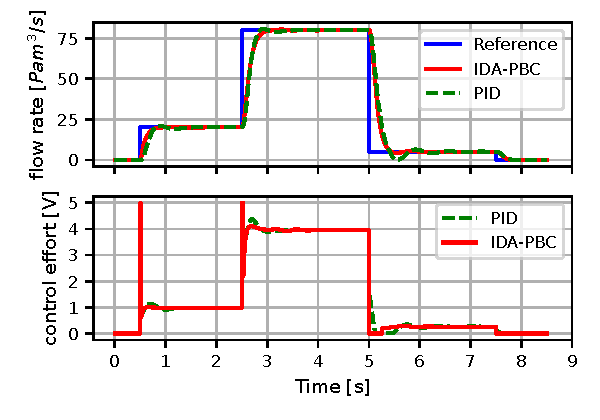
\includegraphics[width=0.4\textwidth]{flow_steps_H2.pdf}
    \caption{Result of IDA-PBC control on high flow valve with $H_2$}
    \label{fig:ctrlsteps_H2}
\end{figure}
\begin{figure}[!ht]
    \centering
    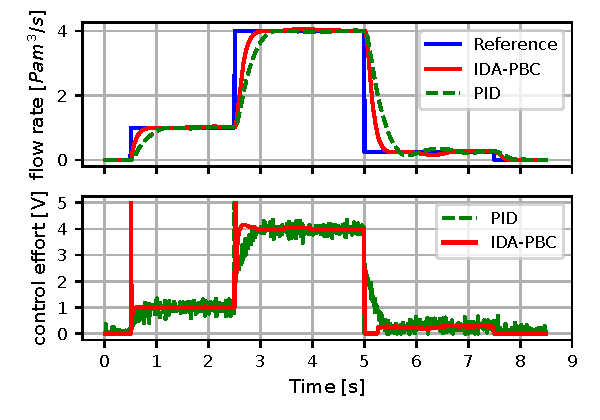
\includegraphics[width=0.4\textwidth]{flow_steps_Ar.pdf}
    \caption{Result of IDA-PBC control on low flow valve with $Ar$}
    \label{fig:ctrlsteps_Ar}
\end{figure}


The resilience of the system to steady state disturbances was also tested. A step force is applied to the valve plunger at $t=3s$, and as can be seen in Figs. \ref{fig:ctrldist_H2} and \ref{fig:ctrldist_Ar} the system converges back to the desired equilibrium.

\begin{figure}[!ht]
    \centering
    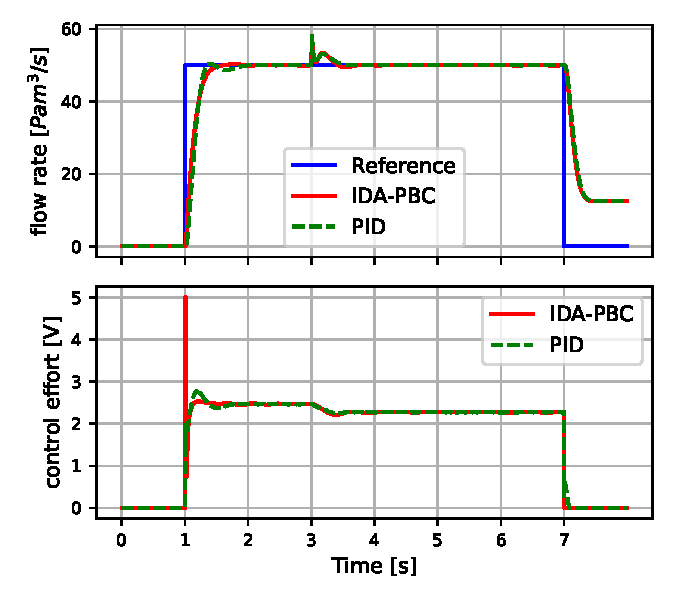
\includegraphics[width=0.4\textwidth]{flow_dist_H2.pdf}
    \caption{High flow valve with step force disturbance at $t=3s$, $H_2$}
    \label{fig:ctrldist_H2}
\end{figure}
\begin{figure}[!ht]
    \centering
    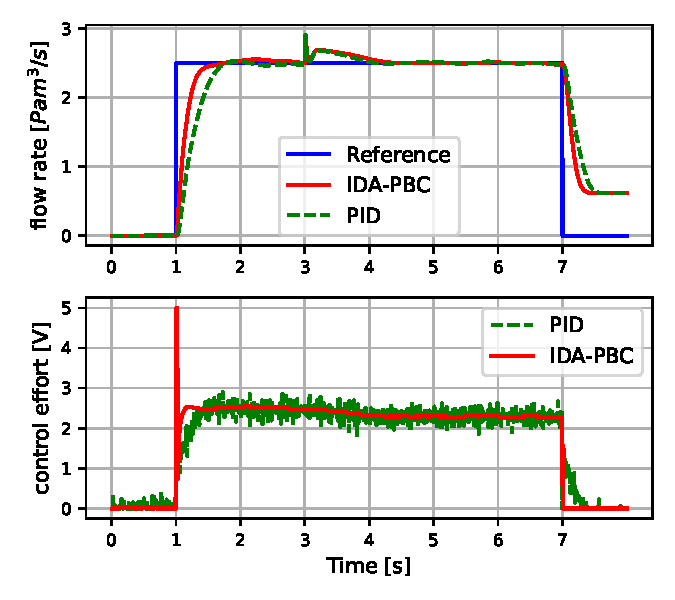
\includegraphics[width=0.4\textwidth]{flow_dist_Ar.pdf}
    \caption{Low flow valve with step force disturbance at $t=3s$, $Ar$}
    \label{fig:ctrldist_Ar}
\end{figure}

The pipe model is then connected to the MFC model in the PCSSP. Fig. \ref{fig:ctrlstep_pipeout} illustrates the flow at the pipe's output for both $H_2$ and $Ar$. The relatively low flow rate of $Ar$ results in a significantly longer delay, exceeding $2.5s$, compared to the shorter delay of approximately $0.5s$ observed for the higher flow rate of $H_2$. This behavior aligns with expected physical phenomena. Furthermore, these observations provide a quantitative constraint on the GIS system's ability to regulate plasma density, which must be carefully considered in the control strategy at ITER.

% * <vu.nmtrang@gmail.com> 11:51:16 11 Mar 2025 UTC+0100:
% may put the following figures into 1 plot, to save space
\begin{figure}[!ht]
    \centering
    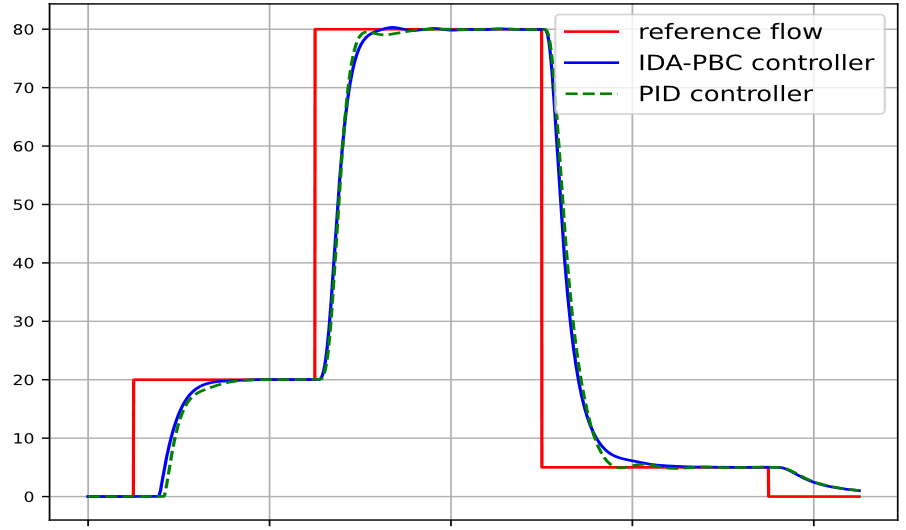
\includegraphics[width=0.35\textwidth]{ctrlsteps_H2_pipeout.png}
    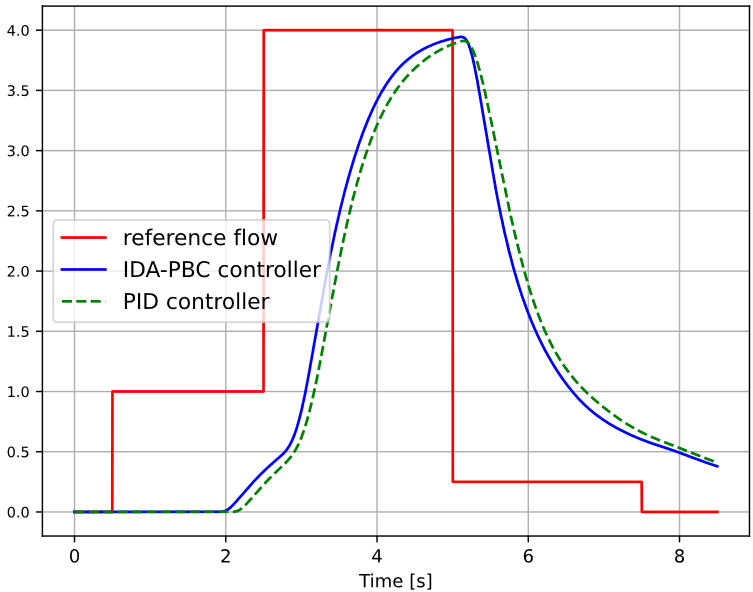
\includegraphics[width=0.35\textwidth]{ctrlsteps_Ar_pipeout.png}
    \caption{Flow at the pipe output for $H_2$ (top) and $Ar$ (bottom)}
    \label{fig:ctrlstep_pipeout}
\end{figure}


\section{Conclusions}\label{sec:conclusion}
This paper presents a dynamic model of solenoid-actuated MFC valves intended for use in the ITER GIS system, as well as a model for the piping connecting the valves to the vacuum vessel. An observer and controller for the MFC valve were developed, tested in simulation, and their performance and robustness to disturbances were successfully validated. The proposed control strategy demonstrates superior effectiveness compared to a PID controller, particularly in scenarios where flow sensor limitations are most significant, such as in the case of low-flow valves, by minimizing overshoot.

\bibliographystyle{IEEEtran} 
\bibliography{refs} % Entries are in the refs.bib file
\end{document}
